%\begin{figure}[h]
%	\centering\includegraphics[width=0.8\textwidth]{fig/figure_4}
%	\caption{Extrem coole Grafik!}
%\end{figure}


% SUBFIGURE
%\begin{figure}[h]
%	\centering
%	\subfigure[]{\includegraphics[width=0.49\textwidth]{fig/2_a_plot}}
%	\subfigure[]{\includegraphics[width=0.49\textwidth]{fig/2_b_plot}}
%	\caption{\textbf{a)} Temperatur des Aluminium Hohlzylinders gegen die Zeit aufgetragen, \textbf{b)} Änderung der Temperatur gegenüber der Temperatur aufgetragen. Jeweils unter Verwendung des Heizdrahtes.}
%	\label{fig:2_1_plot}
%\end{figure}


\section{Einführung}

Das Restgasspektrum wurde wie in der Einführung beschrieben aufgenommen. Es wurde allerdings nicht der ganze Messbereich erfasst, sondern nur der Bereich von 1-50\;u, da fast alle erwarteten Elemente sich in diesem Spektrum befinden.\\
Wie in Abbildung \ref{fig:untergrund_1} zu sehen ist, wurden Peaks bei m = \{1, 2, 16, 17, 18, 19, 28, 32, 44\} u gemessen. Die kleineren Peaks um 18\;u entsprechen dabei dem Cracking-Pattern von Wasser, hierbei handelt es sich also um Bruchmoleküle, die aus dissoziiertem
H$_2$O entstanden.\\
Bei den restlichen Peaks der schwereren Elemente handelt es sich um molekularen Stickstoff (N$_2$, m = 28\;u), molekularen Sauerstoff (O$_2$, m = 32\;u) und Kohlenstoffdioxid (CO$_2$, m = 44\;u).\\

\begin{figure}[h]
	\centering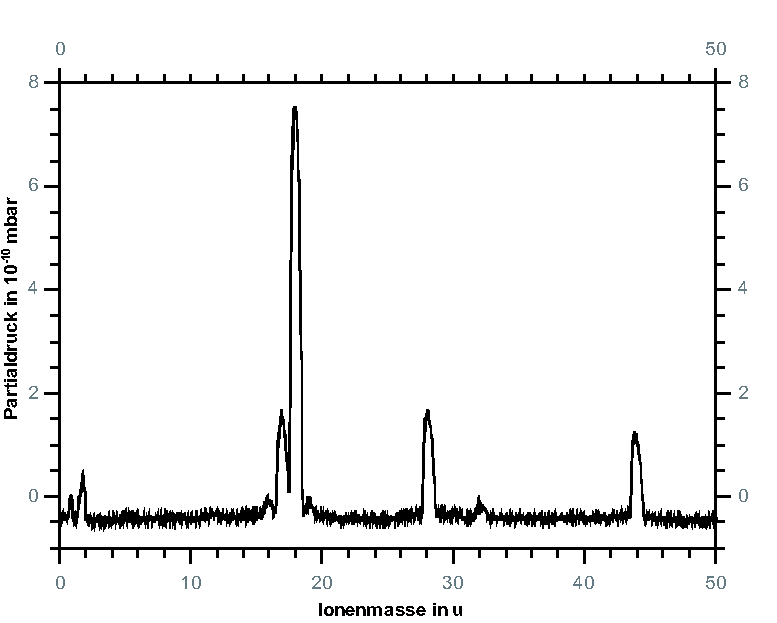
\includegraphics[width=0.8\textwidth]{fig/untergrund_1}
	\caption{Untergrundspektrum des Restgases}
	\label{fig:untergrund_1}
\end{figure}
%TODO: Grafik noch ändern, ist hässlich und die x-Achse ist noch nicht geeicht!

Zur Bestimmung des Auflösungsvermögens wird, wie in der Vorbereitung beschrieben, die z\%-Linienbreite Definition verwendet, wobei z=20 gewählt wurde.\\
Dafür wurde noch einmal mit höherer Abtastrate die Massenbereiche 1-5\;u und 25-30\;u gemessen.\\
Wie erwartet steigt das Auflösungsvermögen mit steigendem m. Dies liegt daran, dass die Linienbreite $\Delta m$ bei unterschiedlichen Massenzahlen hinreichend konstant ist, zumindest immer <1, wobei die Massenzahl monoton steigt.\\

\begin{tabular}{ccc}
	\toprule
	$m$ in u&$\Delta m$ in u&R\\
	\midrule
	2&0.56&3.57\\
	18&0.94&19.15\\
	28&0.89&31.46\\
	\bottomrule
\end{tabular}


\section{Auftrittsenergie von Argon}